\begin{table}[ht]
    \centering
    \caption{\label{tab:failure_modes}Überischt des mit Versagens der Einzelschichten verknüpften Sichheitsrisikos.}
    \begin{tabularx}{\textwidth}{lXXX}
    \toprule
    &\makecell{Pouchfolienversagen\\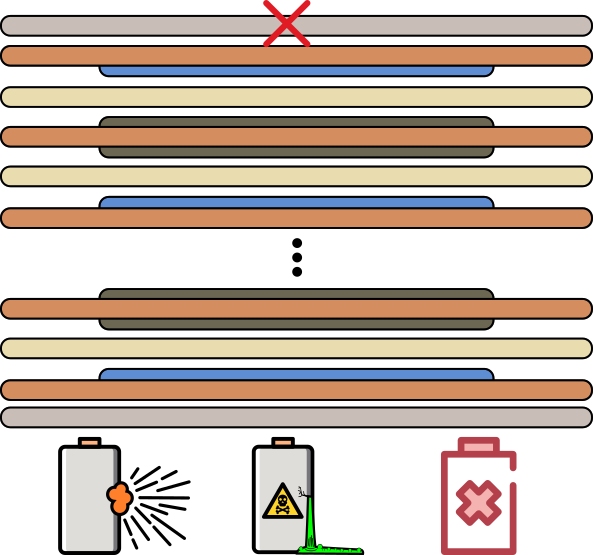
\includegraphics[width=0.2\textwidth]{failure_modes/failure_mode_pouch.png}}
    &\makecell{Elektrodenversagen\\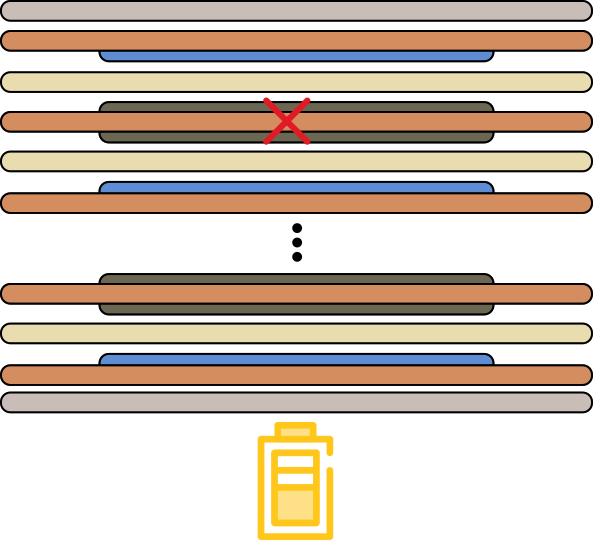
\includegraphics[width=0.2\textwidth]{failure_modes/failure_mode_electrode.png}}
    &\makecell{Separatorversagen\\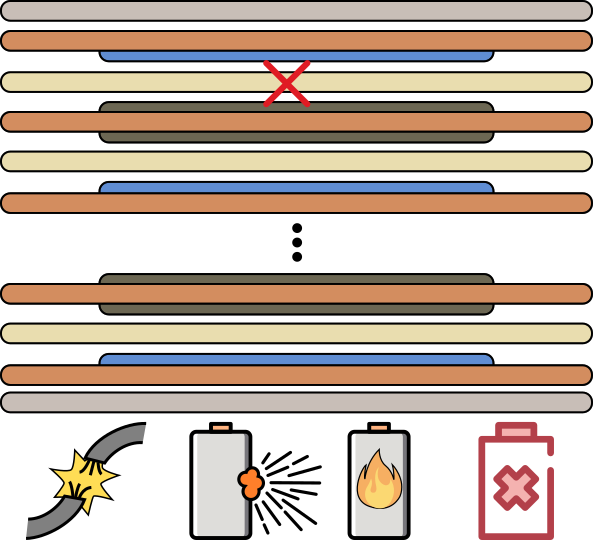
\includegraphics[width=0.2\textwidth]{failure_modes/failure_mode_separator.png}}
    \\
    \midrule
    Funktion
        & Funktionsversagen der gesamten Batterie durch austrocknen
        & Leistungsverlust der Zelle
        & Funktionsversagen der Zelle, je nach Verschaltung auch der gesamten Batterie
    \\
    Brandgefahr
        & kein Risiko
        & kein Risiko
        & Flammenbildung durch Überhitzung
    \\
    Gesundheit
        & hohes Risiko durch austretendes Elektrolyt
        & kein Risiko
        & kein zusätzliches Risiko
    \\
    \bottomrule
    \end{tabularx}\\
    %\noindent{\footnotesize{\textsuperscript{*} Gemessen gegenüber \ce{Li}/\ce{Li+}.}}
\end{table}%